\chapter{外部トリガを用いた応答評価試験}
この章では,外部トリガを用いた粒子線に対する応答評価試験について述べる.\ref{sec:extplan}節で外部トリガを用いた応答評価試験の概要,\ref{sec:extsetup}節で外部トリガでデータ取得をする際のセットアップ,\ref{sec:exthow}節で手順,\ref{sec:extconc}節で取得データ結果を示し,\ref{sec:extsum}節で考察を行なっている.

\section{外部トリガを用いた応答評価試験概要}
\label{sec:extplan}
この節では,Quad Chip RD53Aモジュールに対して行われる品質試験について述べる.\ref{sec:masspro}節で述べたように,現在実機で用いるモジュールを量産するための準備として,プロトタイプ版のASICが4 $\mathrm{Chip}$搭載されたQuad Chip RD53Aモジュールで量産体制の確認が計画されている.この時に,バンプボンディングに異常が無いかを確認するための試験が,外部トリガを用いた応答評価試験である.現在計画されている試験は,クーリングボックスと呼ばれる,温度が低温に維持された小さな箱の中で行い,トリガには前章で述べたHitOR信号ではなく,トリガシンチの信号を外部トリガとして用いる.トリガシンチは箱の上部に取り付けられたソースホルダによって固定され,トリガシンチの信号は,クーリングボックスの外部にある読み出しシステムによって,YARRのDAQへ伝達される.トリガシンチの構成については\ref{sec:extsetup}節で詳しく述べる.計画されている外部トリガを用いた応答評価試験セットアップを図\ref{fig:trigplan}に示す.

\begin{figure}[h]
  \centering
  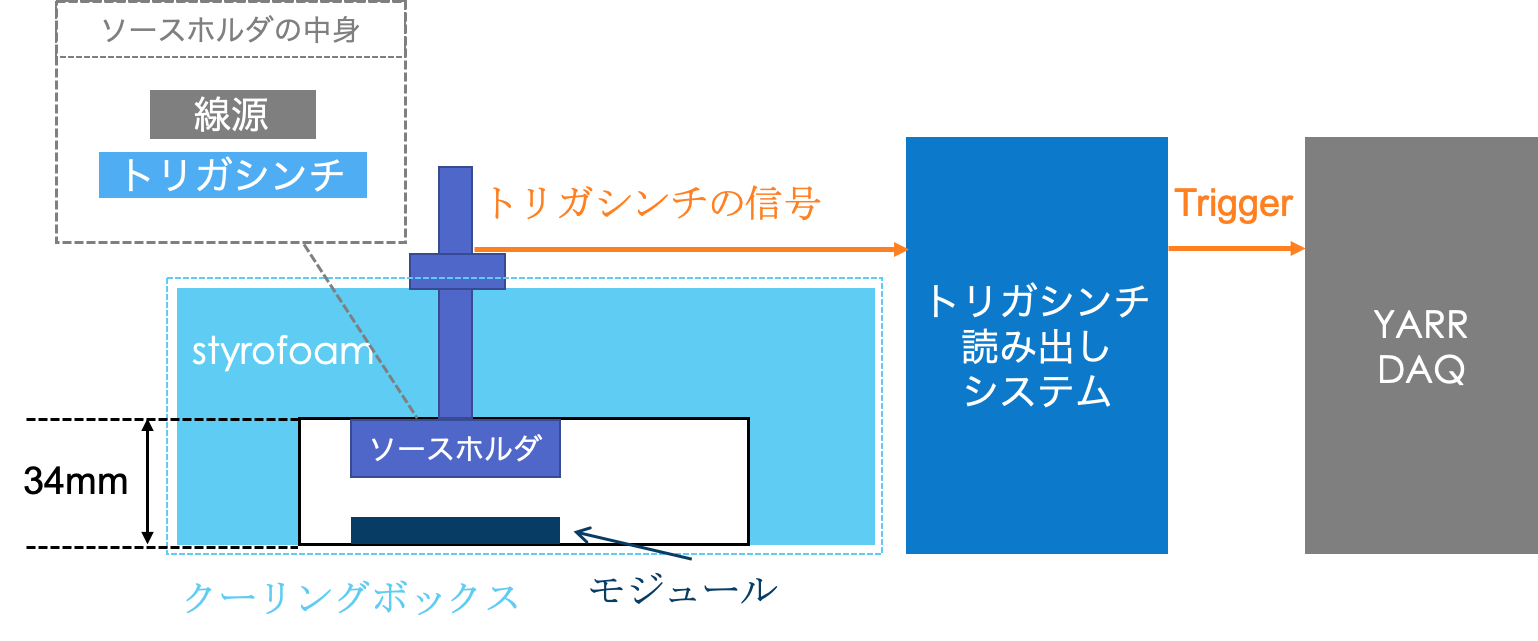
\includegraphics[width=15cm]{./figure/trigplan.png}
  \caption{計画されている外部トリガを用いた応答評価試験セットアップ}
  \label{fig:trigplan}
\end{figure}

計画されているセットアップに近付けるようにして,外部トリガを用いた応答評価試験を行なった.

\section{外部トリガを用いた応答評価試験セットアップ}
\label{sec:extsetup}
今回行なった外部トリガを用いた応答評価試験のセットアップを図\ref{fig:extsetup}に示す.主にセルフトリガの際と変わらず,RD53A搭載のSingle Chip Card(SCC)とFPGAボード,PCを用いて読み出しシステムを構成している.読み出しASICとFPGAボードは,FMC-mDP変換ボードを用いてケーブルにて接続を行い,FPGA内部でASICからのデータ信号の処理を行なった.また,高速通信用インターフェースでPCとFPGAボードを接続し,データ転送を行なった.そして,これらに加え,今回は外部トリガにトリガシンチを用いるため,トリガシンチ,トリガシンチ信号読み出しシステム,ソースホルダが存在する.トリガシンチ信号読み出しシステムのDPコネクタとアダプタカードのport Dが繋げられている.また,将来的にQuad Chipモジュールを読み出すことを考えて,FMC-mDP変換ボードはFPGAボードのHPCコネクタに取り付けられており,FPGAボードにもHPCから信号を受け取れるファームウェアを実装した.HPCはLPCよりも多くの信号が受け取れるコネクタである.\par

\begin{figure}[h]
  \centering
  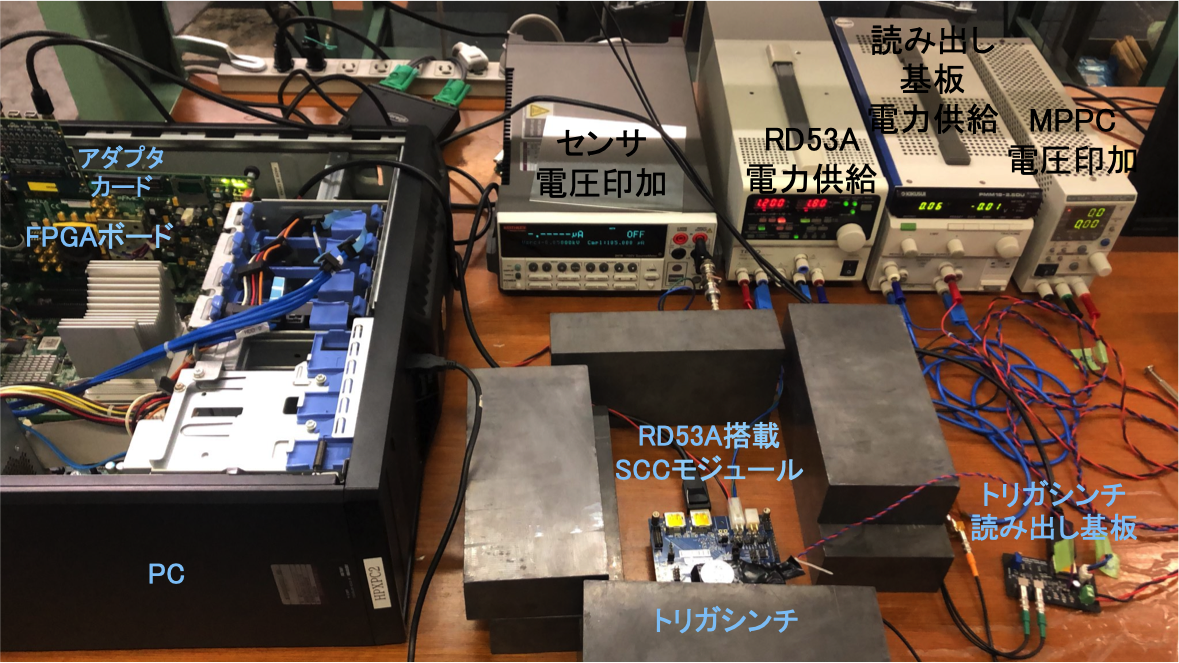
\includegraphics[width=15cm]{./figure/extsetup.png}
  \caption{トリガシンチによるデータ取得のセットアップの様子}
  \label{fig:extsetup}
\end{figure}

\begin{figure}[h]
  \centering
  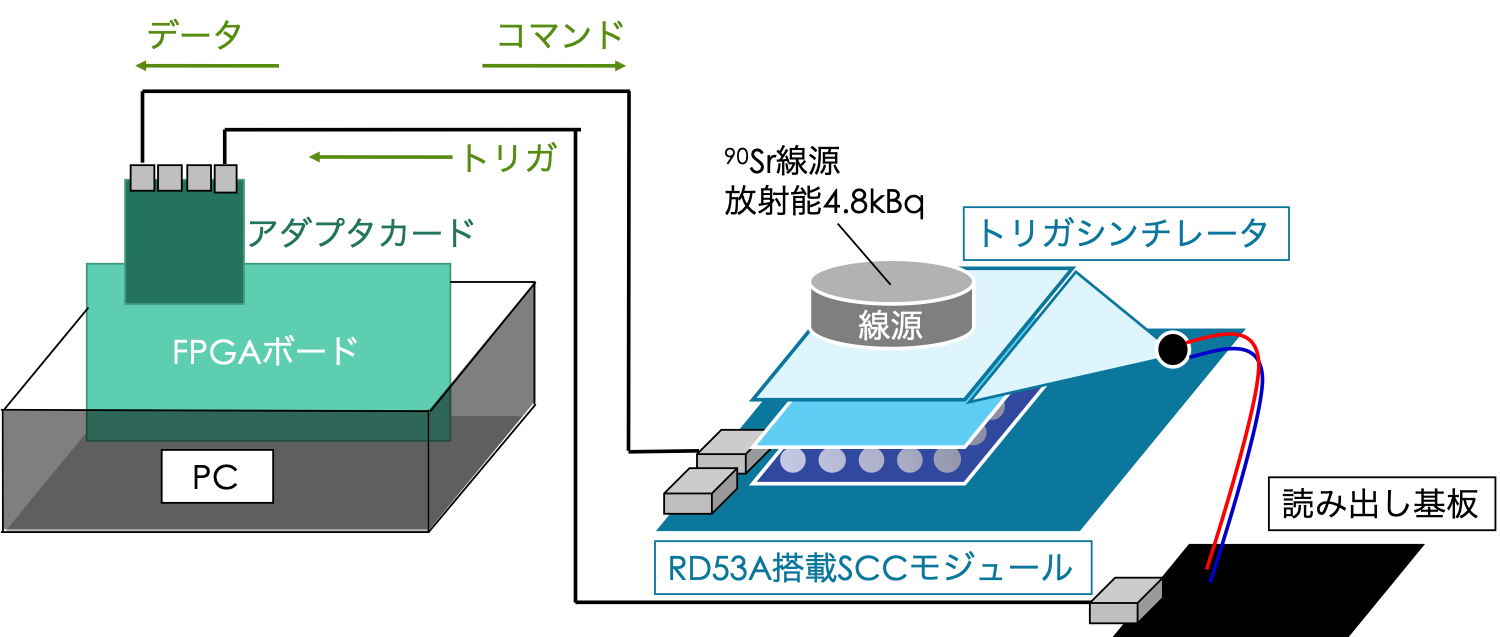
\includegraphics[width=15cm]{./figure/extsetupcab.png}
  \caption{トリガシンチによるデータ取得のセットアップ配線図}
  \label{fig:extsetupcab}
\end{figure}

今回SCCの電源,センサ,読み出し基板,MPPCに印加した電圧を表\ref{tab:extvol}に示す.
\begin{table}[h]
  \centering
  \caption{今回RD53Aとセンサに供給した電圧}
  \begin{tabular} {|l|cc|c|c|c|} \hline
     & RD53A & RD53A & ピクセル & 読み出し & \\ 
     & アナログ回路 & デジタル回路 & センサ & 基板 & MPPC \\ \hline
    印加電圧[$\mathrm{V}$] & 1.80 & 1.80 & -50 & $\pm$ 5.5 & 58\\ \hline
  \end{tabular}
  \label{tab:voltage}
\end{table}


\subsection{トリガシンチ}
今回トリガシンチに使用したシンチレータと,MPPCをシンチレータに取り付けた様子を図\ref{fig:scin}に示す.図中のライトガイドとは,シンチレータに粒子が入射した時に発光した光を効率よくMPPCまで伝えるための部品である.また,\ref{sec:extplan}節でも述べたように,非常にコンパクトな環境での利用を目的としているため,トリガシンチは箱の中,読み出し回路は箱の外で使用される.それに伴って,MPPCの足は約30 $\mathrm{cm}$のケーブルをはんだづけすることで延長し,トリガシンチの信号を箱の外まで伝えられるようにしてある.また,荷電粒子がトリガシンチに遮蔽され,モジュールまで届かなくなることがないように,シンチレータは0.5 $\mathrm{mm}$と非常に薄いものを使用している.シンチレータは光収集率をよくするために,白い紙で覆ったのち,MPPCと共に黒テープで遮光を行なった.その様子を図\ref{fig:trigscin1}に示す.トリガシンチを構成する要素えあるMPPCとシンチレータについて以降述べる.

\begin{figure}[h]
  \centering
  \begin{minipage}[b]{0.45\linewidth}
    \centering
    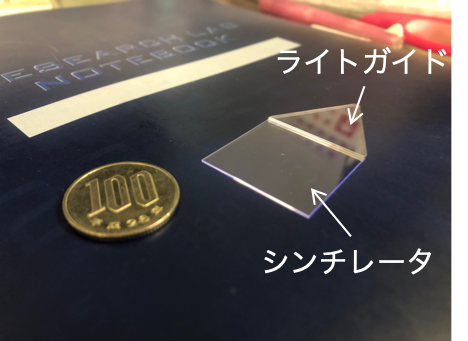
\includegraphics[width=6cm]{./figure/trigscin.png}
    \subcaption{使用したシンチレータとライトガイド}
    \label{fig:scin}
  \end{minipage}
  \begin{minipage}[b]{0.45\linewidth}
    \centering
    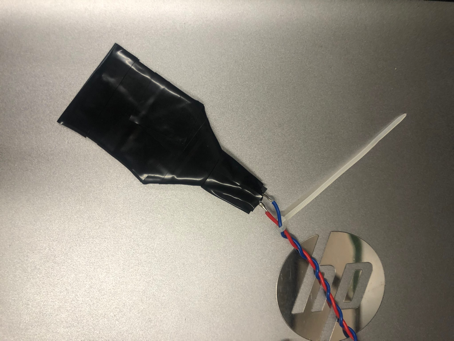
\includegraphics[width=6cm]{./figure/trigscin1.png}
    \subcaption{MPPCを取り付け,遮光したトリガシンチ}
    \label{fig:trigscin}
  \end{minipage}
  \caption{0.5mmのシンチレータの様子}
  \label{fig:trigscin1}
\end{figure}


\subsubsection*{MPPC}
MPPCとは,Silicon Photomultipliers(SiPM)と呼ばれるデバイスの一種であり,複数の半導体光検出器・アバランシェフォトダイオード(APD)から成るフォトンカウンティングデバイスである.本論文で用いたMPPC・HAMAMATSU S13360-1325CSは,$1.3 \times 1.3 \mathrm{mm^2}$の受光面に$25 \times 25 \mathrm{\mu m^2}$のAPDが敷き詰められている.MPPCの構成を図\ref{fig:APD}に示す.

\begin{figure}[h]
  \centering
  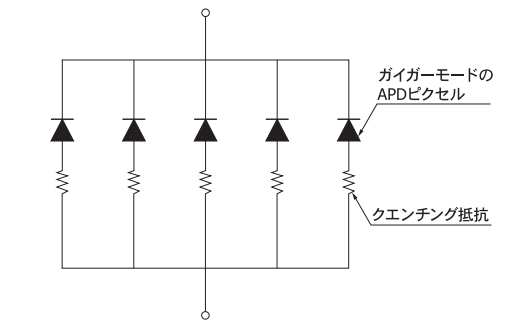
\includegraphics[width=8cm]{./figure/apd.png}
  \caption{MPPCの構成\cite{03handbo69:online}}
  \label{fig:APD}
\end{figure}

全てのAPDの読み出し線,および電圧供給の線は共通していて,全てのAPDピクセルからのシグナルの総和が1つのMPPCからの出力として得られる構造になる.MPPCでは各APDピクセルからの応答が良く揃っているために、総和として出力されるシグナル$Q_{total}$は式\ref{eq:photon}で示されるように光子を受光したピクセル数$N$に1つのAPDから得られるシグナル$Q$をかけた値となる

\begin{eqnarray}
  \label{eq:photon}
  Q_{total} = N \times Q
\end{eqnarray}

受光したピクセル数は、光が微弱である時入射する光量に比例するため, MPPCは非常に高いフォトンカウンティング能力を備えている.

\subsubsection*{プラスチックシンチレータ}
シンチレータとは,放射線のエネルギーを吸収し,内部で励起あるいは電離が起こることで発光する物質である.材質には,無機結晶や液体など様々あるが,本論文では,プラスチックシンチレータを用いた.

%\subsection{トリガシンチの信号読み出し基板}
%本研究を行うにあたって,MPPCからの信号をYARRのDAQシステムのトリガとして使用できるように波形整形できるシステムを作成した.トリガシンチの信号は読み出し基板1で増幅され,コンパレータによってアナログデジタル変換される.その後,ATLYSにてDelayされ,読み出し基板2によってTTLからLVDS変換され,DPコネクタから信号が出力される仕組みである.読み出し基板にDelay機能が実装されていないため,このように2枚の読み出し基板とFPGAボードで構成されている.
%
%\begin{figure}[h]
%  \centering
%  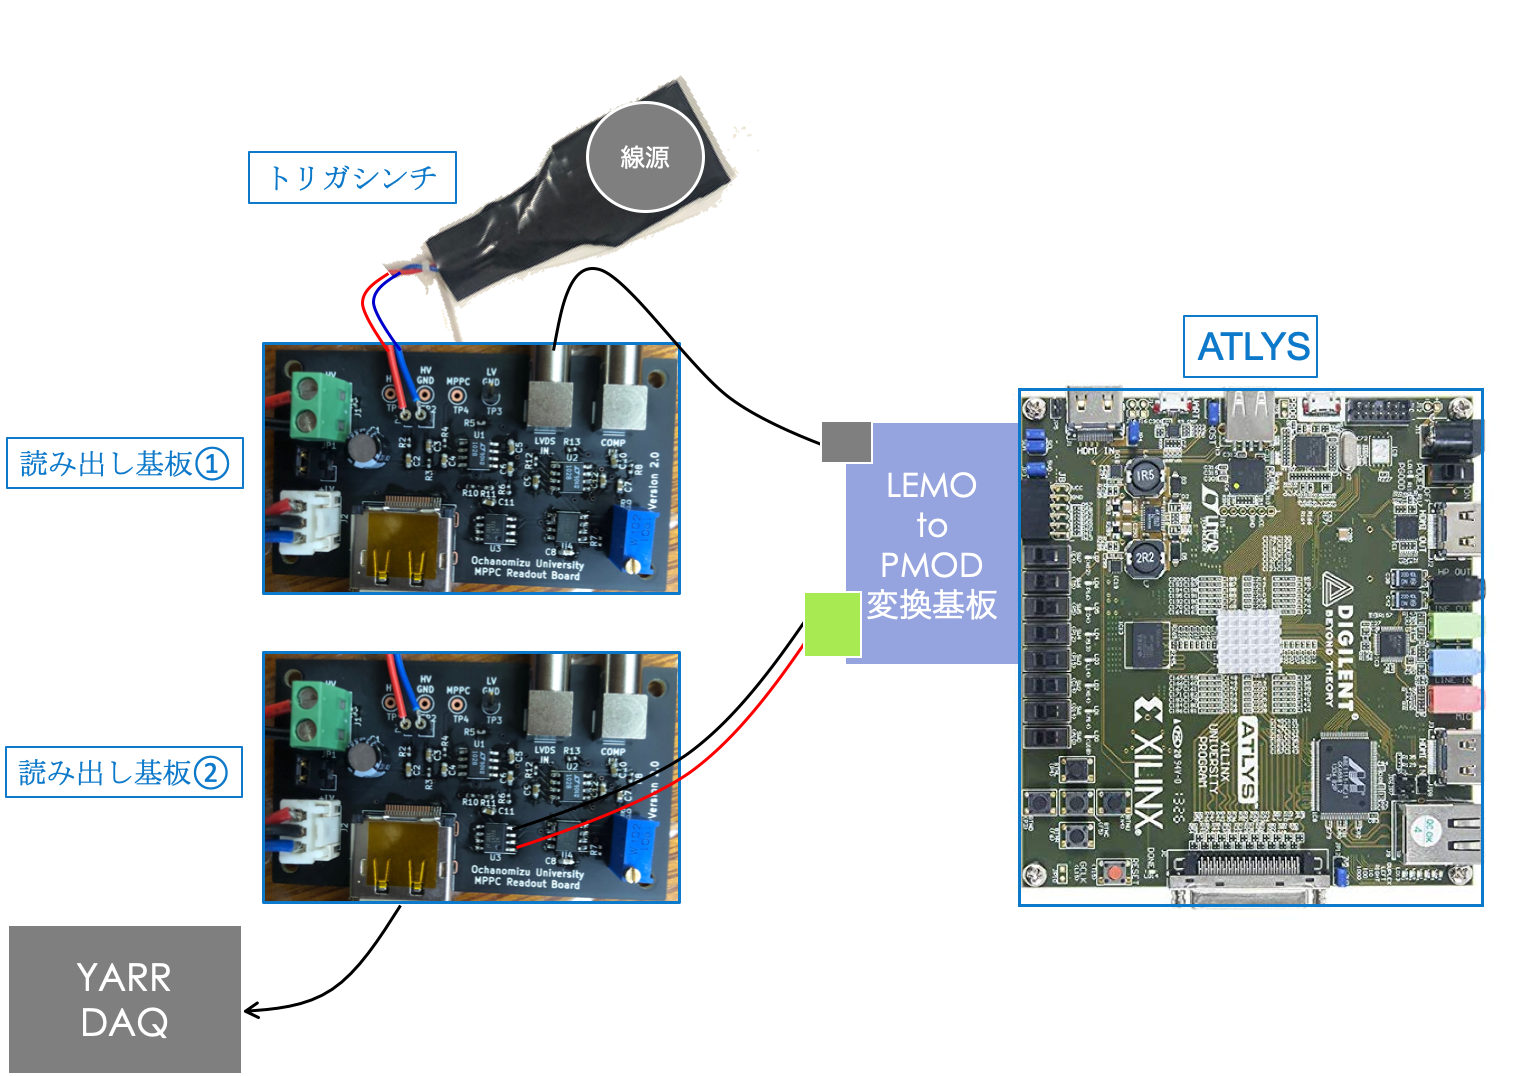
\includegraphics[width=15cm]{./figure/exttriggersetup.png}
%  \caption{トリガシンチの信号を読み出すシステム全体像}
%  \label{fig:exttriggersetup}
%\end{figure}
%
%\begin{figure}[h]
%  \centering
%  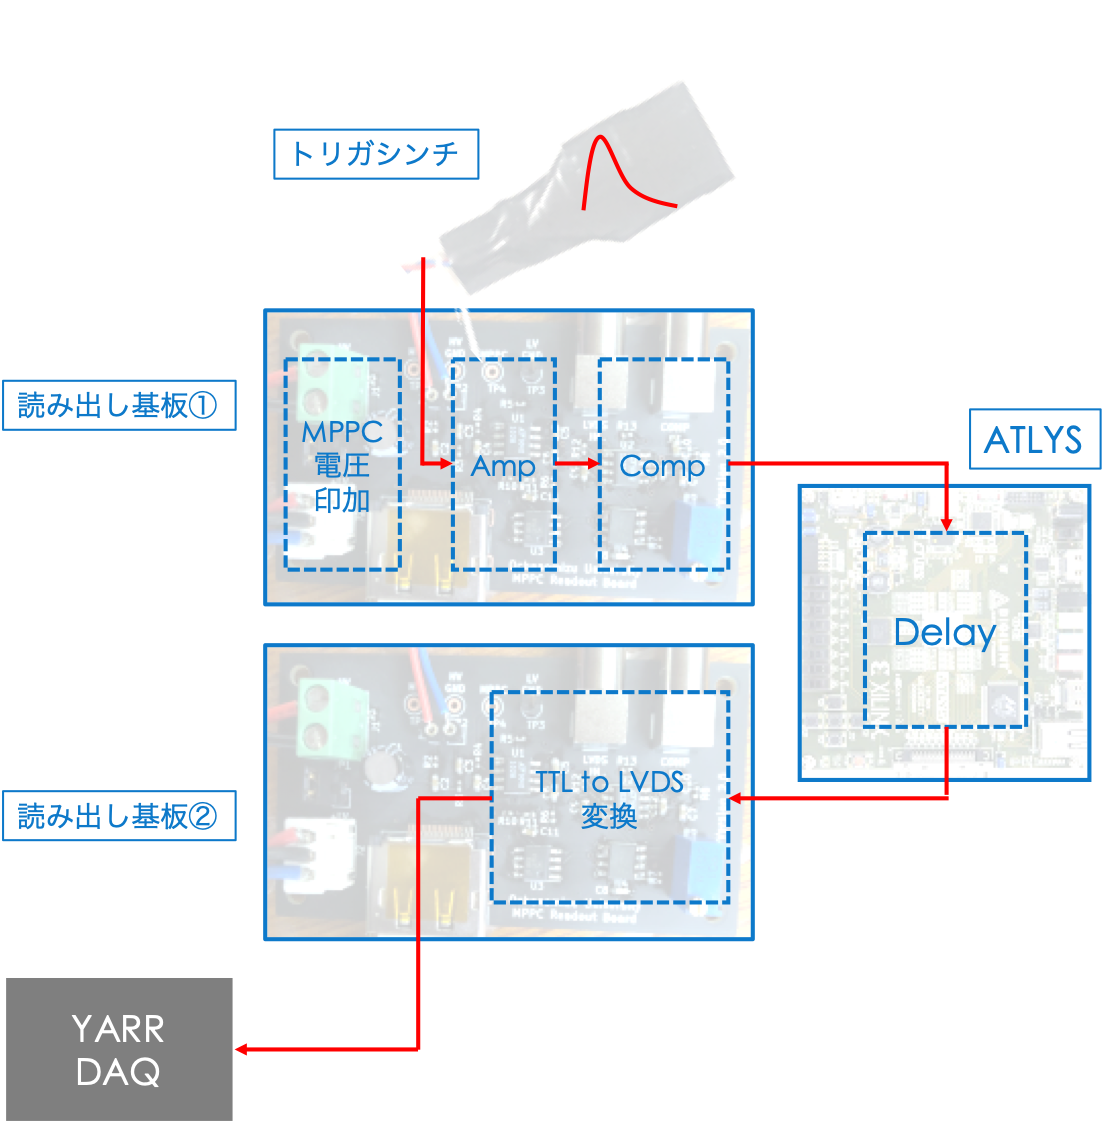
\includegraphics[width=10cm]{./figure/exttriggersignal.png}
%  \caption{トリガシンチの信号がYARR-DAQに伝わるまでの様子}
%  \label{fig:exttriggersignal}
%\end{figure}
%
%
\subsection{読み出し基板}
本研究を行うにあたって,MPPCからの信号を波形整形する基板を作成した.基板を図\ref{fig:pcb}に示す.主に,電圧供給回路,反転増幅回路,コンパレータ回路,LVDS変換回路から構成されている.基板はKiCADというCERN開発のオープンソースプリント基板CADを用いて設計・作成した.LEMO1からは増幅されたMPPCのアナログ信号を,LEMO2からはコンパレータによって閾値電圧と比較することで変換されたデジタル信号を,DPからはTTLだったデジタル信号が変換されてLVDS出力のデジタル信号を読み出すことができる.その3点についてオシロスコープで観測した波形を図\ref{fig:extosiro}に示す.トリガシンチに荷電粒子が入射した信号を得たいため,オシロスコープの様子から,コンパレータの比較電圧は75 $\mathrm{mV}$とした.

\begin{figure}[h]
  \centering
  \begin{minipage}[b]{0.45\linewidth}
    \centering
    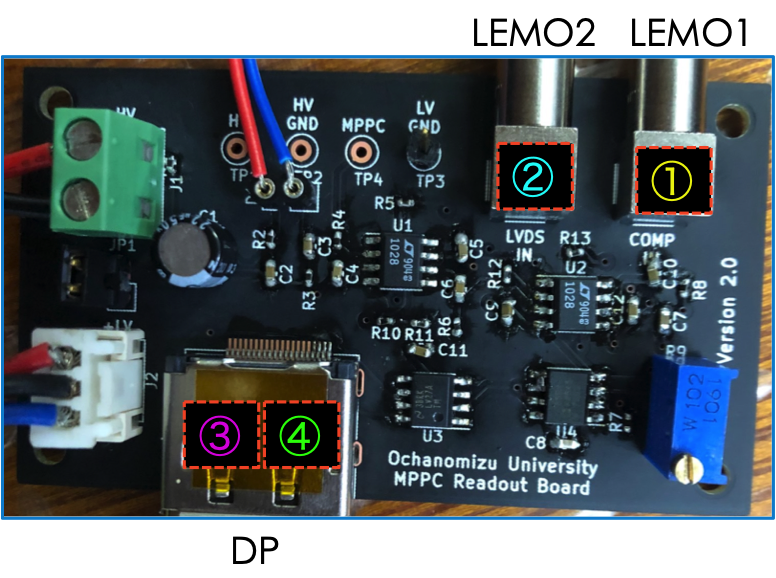
\includegraphics[width=7cm]{./figure/pcb.png}
    \subcaption{基板の様子}
    \label{fig:pcb}
  \end{minipage}
  \begin{minipage}[b]{0.45\linewidth}
    \centering
    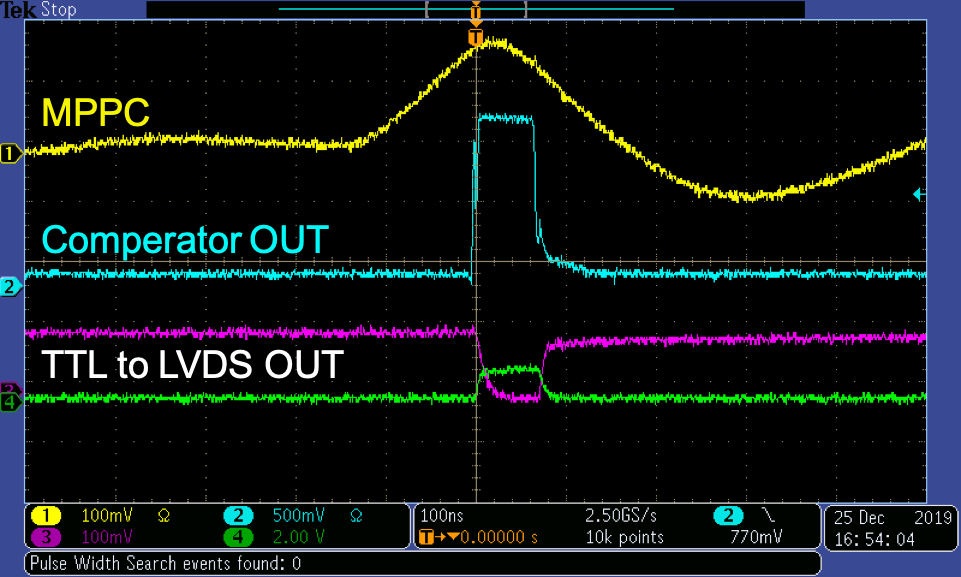
\includegraphics[width=8cm]{./figure/pcbosiro.png}
    \subcaption{動作確認したオシロスコープの様子(コンパレータの比較電圧は150 $\mathrm{mV}$)}
    \label{fig:extosiro}
  \end{minipage}
  \caption{トリガシンチの信号を波形整形する基板}
\end{figure}


\subsection{ソースホルダ}
ソースホルダの外観を図\ref{fig:sourceholder}に示す.クーリングボックス内で使用することを想定し,コンパクトな作りになっている.これは,FreeCADというオープンソース汎用3D CADモデラで設計し,3Dプリンタを用いて作成した.ソースホルダは箱,蓋,軸,留め具の4パーツに分かれていて,蓋の部分には線源を固定するための窪みが存在する.

\begin{figure}[h]
  \centering
  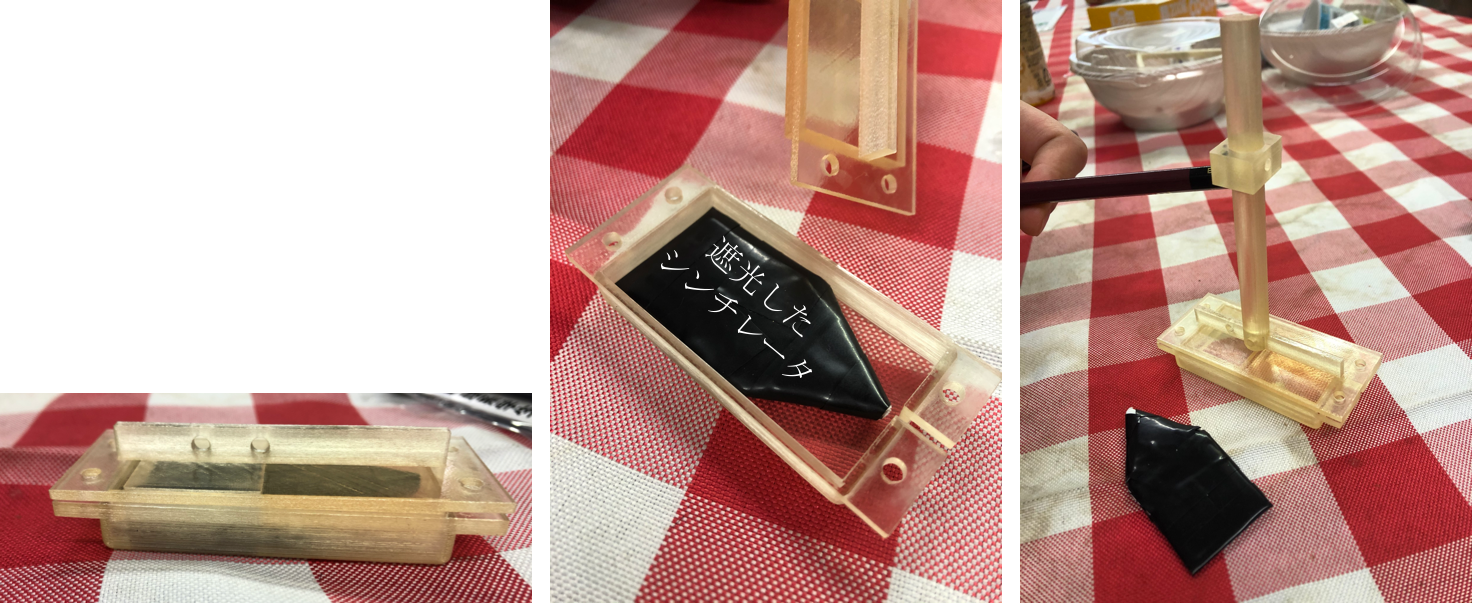
\includegraphics[width=15cm]{./figure/sourceholder.png}
  \caption{ソースホルダの様子}
  \label{fig:sourceholder}
\end{figure}

\section{応答評価試験手順}
\label{sec:exthow}
%まず,前章で述べたようなトリガシンチの信号がFPGAまで伝達され,処理されているかの確認を行った.その確認の様子を図に\ref{fig:extwf}に示す.
%\begin{figure}[h]
%  \centering
%  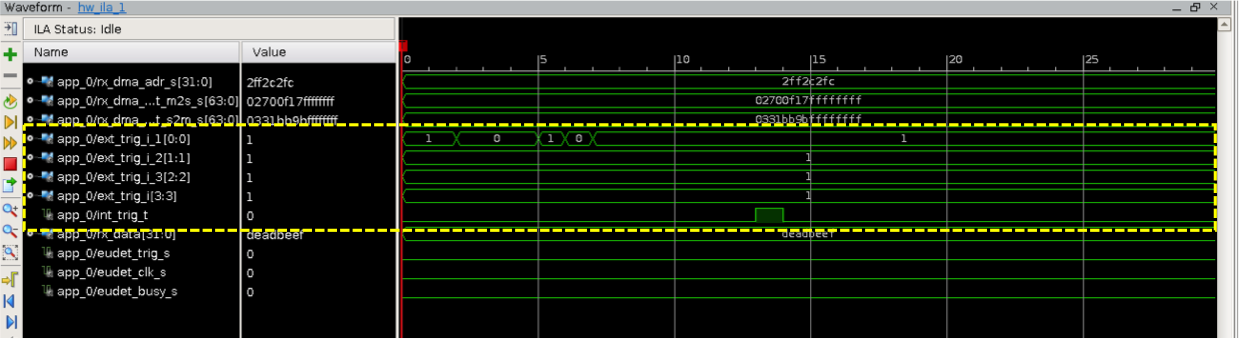
\includegraphics[width=17cm]{./figure/extWF.png}
%  \label{fig:extwf}
%  \caption{VivadoのLogic Analyzerでトリガシンチからの信号を確認した様子}
%\end{figure}

%今回は''ext\_trig\_i[0:0]''にのみ信号を入力しているため,その部分のみが0から1へと変化している.また,''int\_trig''も0から1に変化していることから,ファームウェアにてトリガシンチの信号の受信・処理が正常に行われていることが確認できる.\par
第3章で述べたような動作確認を行ったのち,Latency Scanを行なった.実際の応答試験では,線源とモジュールの間にトリガシンチを配置するが, 荷電粒子がトリガシンチに遮られ,ASICまで届かないことを避けるため,Latency Scanの際には,線源とトリガシンチの間にモジュールを配置した.また,荷電粒子によるデータよりもノイズのデータを多く取得することを防ぐために,Diff FEの上半分,バイアス構造を持つ部分は全て非使用に設定した.Latency Scanの結果を図\ref{fig:exttriglatency}に示す.シンチレータと無関係の光子にMPPCが反応することや,ASICのDiff FE以外を通過した粒子が存在することから,1つの''LatencyConfig''値のトリガ数に対する取得イベント数が図\ref{fig:latencydist}よりも大きく減少しているのがわかる.しかし,この結果で1イベント取得されている''LatencyConfig''値・205でデータ取得した時とそこから離れた値である0でデータ取得を行った時のデータの差から''LatencyConfig''値を211を正しい''LatencyConfig''値と判断した.

\begin{figure}[h]
  \centering
  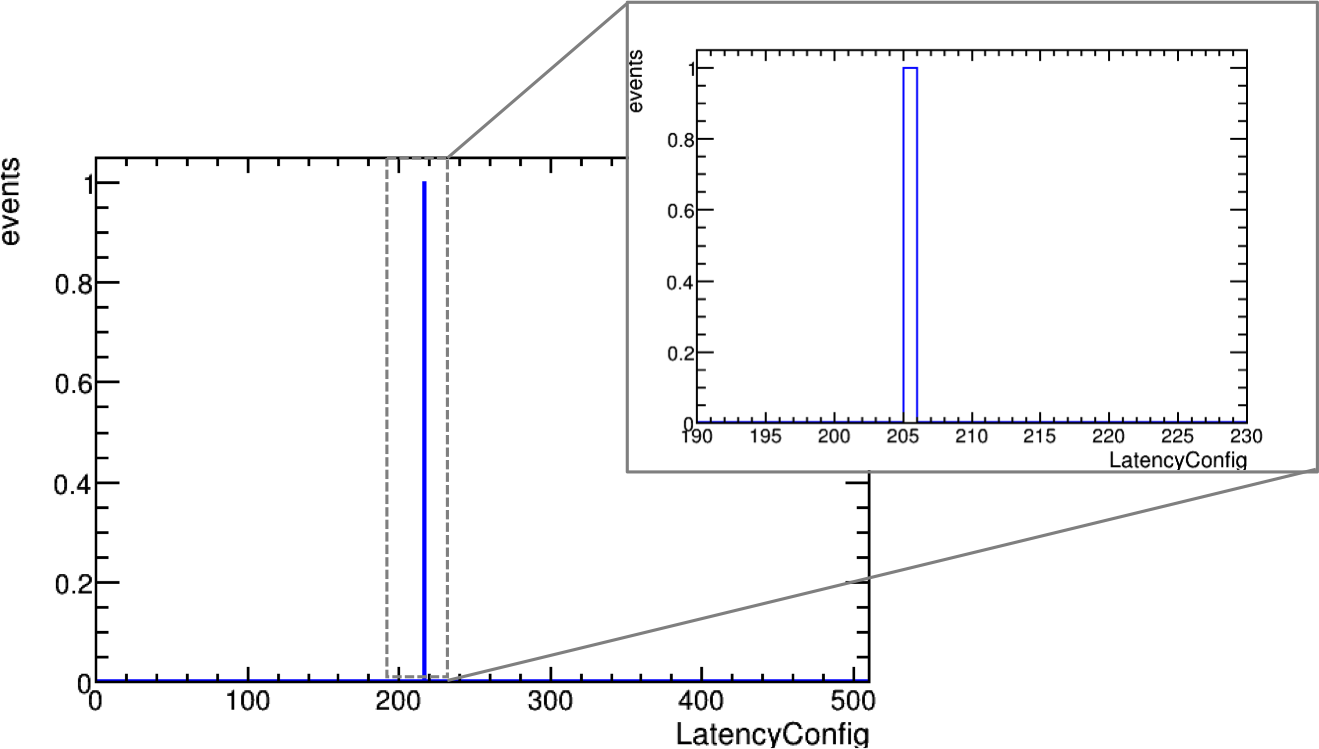
\includegraphics[width=14cm]{./figure/ExtLatencyDist.png}
  \caption{トリガシンチの場合の''LatencyConfig''値とL1ID $== 7$だったイベント数の関係}
  \label{fig:exttriglatency}
\end{figure}

Latencyを合わせた上で,図\ref{fig::extsetup}のセットアップで,以下の3つのトリガ生成方法でデータ取得を行う.
\begin{enumerate}
\item 200 $\mathrm{kHz}$でトリガを生成し,データ取得を行う(ランダムトリガ)
\item 線源を置かない状態でセルフトリガによるデータ取得を行う
\item 線源を置いた状態でセルフトリガによるデータ取得を行う
\end{enumerate}


\section{応答評価試験結果}
\label{sec:extconc}
3つのトリガ生成方法で得られたデータのトリガ数とヒット数を表\ref{tab:self}に示す.

\begin{table}[h]
  \centering
  \caption{トリガ生成方法に対する得られたヒット数とトリガ数}
  \begin{tabular} {l|ccc} \hline
    トリガ生成方法 & ランダムトリガ & セルフトリガ(線源なし) & セルフトリガ(線源あり) \\ \hline
    ヒット数 & & & 3599457 \\
    トリガ数 & $6 \time 10^6$ & 4193685 & 4056311 \\ \hline
  \end{tabular}
  \label{tab:selfpara}
\end{table}

\section{考察}
\subsection*{トリガ生成方法と取得されるデータの内容}
3つのトリガ生成方法による取得されるデータの内容の違いについて表\ref{tab:selfdata}に示す.

\begin{table}[h]
  \centering
  \caption{トリガ生成方法と取得されるデータの内容}
  \begin{tabular} {l|ccc} \hline
    & ランダムトリガ & 外部トリガ(線源なし) & 外部トリガ(線源あり) \\ \hline
    トリガ生成方法 & 200 $\mathrm{kHz}$のトリガ & センサの信号でトリガ生成 & センサからの信号でトリガ生成 \\ \hline
    取得される & 無関係なトリガで & 無関係なトリガで & 無関係なトリガで\\
    データの内容 & 得られるヒット & 得られるヒット & 得られるヒット \\
    & & & 荷電粒子の信号\\ \hline
  \end{tabular}
  \label{tab:extdata}
\end{table}

これより,ランダムトリガによるデータ取得と,線源を置かない時の外部トリガによるデータ取得では,同じデータが取得されることがわかる.よって,線源ありの外部トリガによって取得されたデータから,無関係なトリガで得られるヒットの影響を除くことで荷電粒子からの信号を見積もりたい.以降,ランダムトリガで取得されたデータと,線源ありの外部トリガで取得されたデータにのみ着目する.

\subsection*{荷電粒子からの信号の見積もり}
荷電粒子からの信号を見積もるために,各ピクセルが得たヒット数に着目する.i番目のピクセルに対して,表\ref{tab:selfpara}のように値を定める.

\begin{table}[h]
  \centering
  \caption{i番目のピクセルに対して得られる値}
  \begin{tabular} {l|ccc} \hline
    & ランダムトリガ & セルフトリガ(線源あり) \\ \hline
    ヒット数 & $N_{\mathrm{i.bg}}^{\mathrm{random}}$ & $N_{\mathrm{i}}^{\mathrm{ext}}$ \\
    トリガ数 & $M_{\mathrm{i.bg}}^{\mathrm{random}}$ & $M_{\mathrm{i}}^{\mathrm{ext}}$ \\
    トリガ数に対するヒット数 & $R_{\mathrm{i.bg}}^{\mathrm{random}}$ & $R_{\mathrm{i}}^{\mathrm{ext}}$ \\\hline
  \end{tabular}
  \label{tab:extpara}
\end{table}

この時,$N_{\mathrm{i}}^{\mathrm{ext}}$に対して,ランダムトリガによる影響を除いたもの$N_{\mathrm{i.sig}}$を式\ref{eq:extphits}のように表す.$N_{\mathrm{i.sig}}$が荷電粒子による信号の見積もりである.
  
\begin{eqnarray}
  \label{eq:extphits}
  N_{\mathrm{i.sig}} &=& N_{\mathrm{i}} - \mathrm{i.Background} \\
  \mathrm{i.Background} &=& \left(\frac{N_{\mathrm{i.bg}}^{\mathrm{ext}}}{M_{\mathrm{i.bg}}^{\mathrm{ext}}} + \frac{N_{\mathrm{i.bg}}^{\mathrm{random}}}{M_{\mathrm{i.bg}}^{\mathrm{random}}} \right) \times M_{\mathrm{i}}^{\mathrm{ext}}
\end{eqnarray}

$N_{\mathrm{i}}$と$N_{\mathrm{i.sig'}}$1ピクセルあたりのヒット数分布の違いを図\ref{fig:exthitsperpix1}に示す.
\begin{figure}[h]
  \centering
  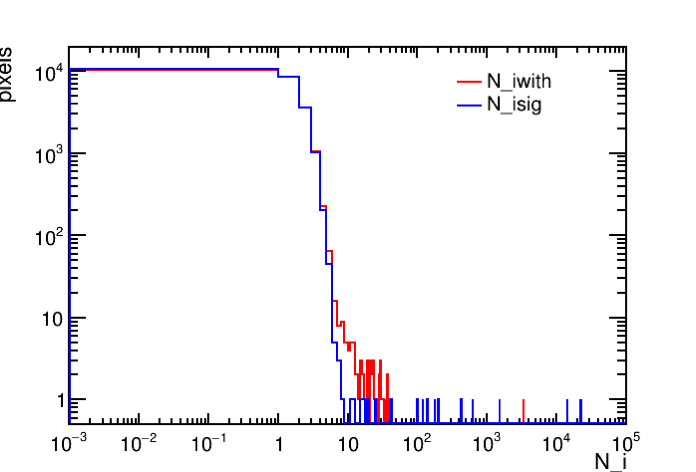
\includegraphics[width=10cm]{./figure/exthitperpix.png}
  \caption{1ピクセルあたりのHit数分布}
  \label{fig:exthitfreq}
\end{figure}

$N_{\mathrm{i}}$と$N_{\mathrm{i.sig}}$1ピクセルあたりのヒット数分布の推移を図\ref{fig:exthitsperpix1bfaf}に示す.横軸が$N_{\mathrm{i}}$で縦軸が$N_{\mathrm{i.sig}}$を示していて,$N_{\mathrm{i}}=10 \mathrm{Hits}$あたりの分布は,$N_{\mathrm{i.sig}}$では0に変化しているピクセルも多く,$N_{\mathrm{i}}$に対するランダムトリガによるヒットの割合が高いことがわかる.
\begin{figure}[h]
  \centering
  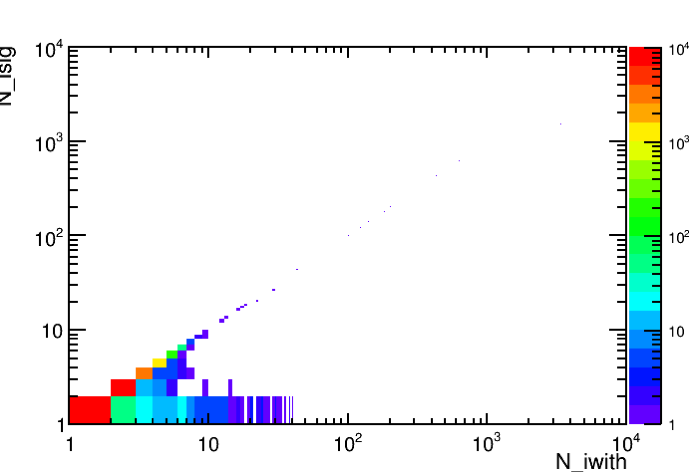
\includegraphics[width=10cm]{./figure/exthitperpixbfaf.png}
  \caption{1ピクセルあたりのHit数分布の推移}
  \label{fig:exthitfreq}
\end{figure}

最終的に得られた荷電粒子の信号$N_{\mathrm{i.sig}}$の分布はポアソン分布式\ref{eq:poisson}に従うので,フィッティングを行い,平均ヒット数を求めた.フィッティングを行なった様子を図\ref{fig:extfit}に示す.

\begin{eqnarray}
  \label{eq:poisson}
  P(x) = \frac{\lambda^x e^{-\lambda}}{x!} (\lambda:\mathrm{const})
\end{eqnarray}

\begin{figure}[h]
  \centering
  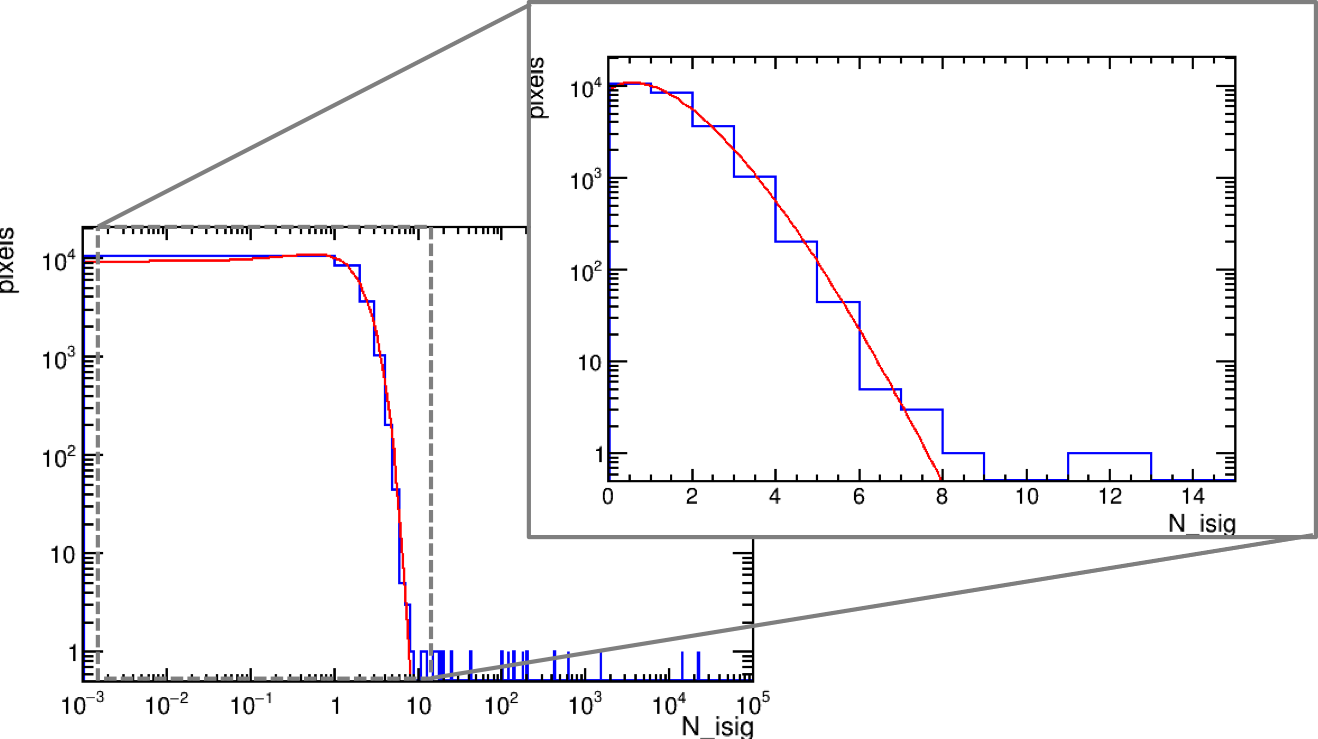
\includegraphics[width=15cm]{./figure/extfit.png}
  \caption{$N_{\mathrm{i.sig}}^{\mathrm{ext}}$の分布をポアソン分布でフィットした様子}
  \label{fig:exthitfreq}
\end{figure}

フィットの結果より,30分のセルフトリガによる応答評価試験で得られる1ピクセルあたりの平均ヒット数は1.10 $\mathrm{Hits/pixel}$と求められた.品質評価に必要なヒット数50 $\mathrm{Hits/pixel}$を得るためには,およそ6.25日かかることがわかった.

\subsection*{全ヒット数に対する荷電粒子によるヒット数}
全ヒット数$N^{\mathrm{ext}}$と,背景事象によるヒット数$N_{\mathrm{bg}}^{\mathrm{ext}}$,荷電粒子によるヒット数$N_{\mathrm{sig}}^{\mathrm{ext}}$の定義を式\ref{eq:extallhits}に示す.

\begin{eqnarray}
  N^{\mathrm{ext}} &=& \sum^{\mathrm{allpixels}} N_{\mathrm{i}} \\
  N_{\mathrm{bg}}^{\mathrm{ext}} &=& \sum^{\mathrm{allpixels}} N_{\mathrm{i.bg}}^{\mathrm{random}} \\
  N_{\mathrm{sig}}^{\mathrm{ext}} &=& \sum^{\mathrm{allpixels}} N_{\mathrm{i.sig}}^{\mathrm{ext}}
\end{eqnarray}

外部トリガによる応答評価試験で得られた$N^{\mathrm{ext}}$に対する$N_{\mathrm{sig}}^{\mathrm{ext}}$の割合とヒットレートを表\ref{tab:extp}に示す.
\begin{table}[h]
  \centering
  \caption{3時間で得られた荷電粒子のヒット数}
  \begin{tabular} {l|ccc} \hline
    time:10800[sec]& $N^{\mathrm{ext}}$ & $N_{\mathrm{bg}}^{\mathrm{ext}}$ & $N_{\mathrm{sig}}^{\mathrm{ext}}$ \\ \hline
    ヒット数 & 591115 & 4620 & 586495 \\
    & (100 \%) & (0.8 \%) & (99.2 \%) \\ \hline
    ヒット数/time & 54.7 $\mathrm{Hz}$ & 0.9 $\mathrm{Hz}$ & 54.3 $\mathrm{Hz}$ \\ \hline
  \end{tabular}
  \label{tab:extp}
\end{table}

荷電粒子によるヒットレート(ヒット数/time)は54.3 $\mathrm{Hz}$と低い結果になっているが,$N\_{\mathrm{ext}}$に対する$N_{\mathrm{i.sig}}^{\mathrm{ext}}$の割合は99.2 \%と非常に高い結果となった.

\subsection*{ヒットが存在したイベント数}
全トリガ数$M^{\mathrm{ext}}$に対する,ヒットが存在しなかったイベント数$M_{\mathrm{emp}}^{\mathrm{ext}}$と,存在したイベント数$M_{\mathrm{data}}^{\mathrm{ext}}$の割合とトリガレートを表\ref{tab:extr}に示す.

\begin{table}[h]
  \centering
  \caption{全トリガ数と対するヒットが存在したイベント数の割合}
  \begin{tabular} {l|ccc} \hline
    time:1800[sec] & $M^{\mathrm{ext}}$ & $M_{\mathrm{data}}^{\mathrm{ext}}$ & $M_{\mathrm{emp}}^{\mathrm{ext}}$ \\ \hline \hline
    トリガ数 & 918246 & 278687 & 639559 \\
     & (100 \%) & (30.3 \%) & (69.7 \%) \\ \hline
    トリガ数/time & 85.0 $\mathrm{Hz}$ & 25.8 $\mathrm{Hz}$ & 59.2 $\mathrm{Hz}$ \\ \hline
  \end{tabular}
  \label{tab:extr}
\end{table}

$M^{\mathrm{ext}}$に対する$M_{\mathrm{data}}^{\mathrm{ext}}$の割合は30.3 \%と,ほとんどのトリガに対して,ヒットのデータが取得できていないことがわかった.これは,トリガシンチレータで荷電粒子が止まってしまったり,トリガシンチレータに入射してもセンサに入射しなかったりすることが原因と考えられる.

